\documentclass[10pt,a4paper]{article}
\usepackage[latin1]{inputenc}
\usepackage{
    amsmath, 
    amssymb, 
    amsthm, 
    amsfonts,
    latexsym,
    graphicx,
    subfig,
    comment,
    url,
    fullpage,
    setspace,
    alltt,
    calc
}
\usepackage{hyperref}

\setlength\fboxsep{4mm}
\setlength\fboxrule{0pt}

\newcommand{\paramtable}[1]{\begin{tabular}{p{4cm}p{16cm}}#1\end{tabular}}

\newenvironment{paramlist}
{\begin{list}{}{
    \renewcommand{\makelabel}[1]{\texttt{##1}\hfil}
    \setlength{\labelwidth}{3cm}
    \setlength{\leftmargin}{\labelwidth+\labelsep}
    }
}
{\end{list}}

% Code examples
% For single line code snippets
\newcommand{\excode}[1]{\begin{quote}\begin{alltt}#1\end{alltt}\end{quote}}
\newcommand{\exnotn}[1]{\begin{quote}\begin{alltt}\normalfont #1\end{alltt}\end{quote}}

% For multiline code snippets
\newenvironment{egcode}
{\begin{quote}\begin{alltt}}
{\end{alltt}\end{quote}}

% Multiline notations/algorithms
\newenvironment{egnotn}
{\begin{quote}\begin{alltt}\normalfont}
{\end{alltt}\end{quote}}

\newcommand{\tss}[1]{\textsuperscript{#1}}

% References
\newcommand{\fig}[1]{Figure~\ref{fig:#1}} 
\newcommand{\tab}[1]{Table~\ref{tab:#1}}
\newcommand{\chap}[1]{Chapter~\ref{chap:#1}}
\newcommand{\sect}[1]{Section~\ref{sec:#1}}
\newcommand{\algo}[1]{Algorithm~\ref{alg:#1}}
\newcommand{\apdx}[1]{Appendix ~\ref{sec:#1}}                        
\newcommand{\thmref}[1]{Theorem~\ref{thm:#1}}
\newcommand{\lemref}[1]{Lemma~\ref{lem:#1}}
\newcommand{\corref}[1]{Corollary~\ref{cor:#1}}
\newcommand{\eqnref}[1]{Equation~\ref{eqn:#1}}

% Shorthand formatting
\newcommand{\ben}{\begin{enumerate}}
\newcommand{\een}{\end{enumerate}}
\newcommand{\bit}{\begin{itemize}}
\newcommand{\eit}{\end{itemize}}
\newcommand{\bvb}{\begin{verbatim}}
\newcommand{\evb}{\end{verbatim}}
\newcommand{\ttt}[1]{\texttt{#1}}
\newcommand{\vpad}{\vspace{8pt}}


\begin{document}

\title{Simulator manual}
\author{James Hanlon\\\ttt{hanlon@cs.bris.ac.uk}}
\date{\today}
\maketitle

This document describes a software network simulator. The simulator is
\emph{cycle-based} and models \emph{flit-level} communication. It is intended to
simulate arbitrary network topologies and routing algorithms based on
\emph{virtual channel} (VC) \emph{wormhole flow-control}. It is based on the
\emph{BookSim}\footnote{\url{http://nocs.stanford.edu/cgi-bin/trac.cgi/wiki/Resources/BookSim}}
software simulator accompanying \cite{Dally03}. It is assumed the reader is
familiar with the concepts presented in the book.

\section{System architecture}

Cycle-based means that all network components are tied to a global clock and are
synchronously updated each time-step.  The updates are generally performed in
two phases. The first phase reads some input state and computes some output
values as a function of these. The second phase copies each components output
value into the inputs of the connected components. 

A network is composed of nodes and links. The arrangement of link connections
between nodes determines the topology. Each node contains a processor which acts
as a source and sink for packets, and a router which forwards or queues incoming
flits to an output port or towards the processor if it is the destination.  If
flit generation is less than flit reception then source queues will grow and
network will become saturated. Otherwise, the network will be in a \emph{stable}
state.

\subsection{Nodes}

A \emph{node} is comprised of a \emph{router} (or switch) and a
\emph{processor}.  The router is at the heart of the simulator. It simulates a
non-blocking crossbar with input-buffered VCs. It takes 1 cycle to transfer a
flit from an input to an output buffer. VCs are used for flow control and as a
resource for some protocols and the number available is a simulation parameter.
Credit-based flow control is used to provide \emph{buffer management} and
\emph{back-pressure}.

The processor generates messages according to the traffic pattern and injection
process, and to consume messages sent by other nodes. It is connected to the
router by its own input and output ports which each have only a single virtual
channel. 

\subsection{Links}

Links are used both to connect routers together and the processor the
router. Links are unidirectional but are modeled to contain a second signal
traveling in the opposite direction as the data to transmit the credit messages
back upstream. Links have an associated propagation delay in cycles, modeling
the physical propagation of electrical or optical signals along a cable or
fiber. If the delay is $d$ cycles then the link can simultaneously carry $d$
flits and $d$ credits in either direction at different stages along the journey.

\section{Compilation and Running}

The simulator is written in Java and can be built and run from source code with
the included Makefile, by running \ttt{make}. The simulator can then be run by
setting the classpath variables (\ttt{make classpath}) and executing
\excode{java sim.Main \(\langle\)config\(\rangle\).cfg} or by running the
command \ttt{make run} which both sets-up the classpath and executes the
program.

\subsection{Dependencies}

The simulator uses the JGraphT\footnote{\url{http://jgrapht.sourceforge.net/}}
library. The library jar must be included in the class path to build and run. The
location of this can be specified in the Makefile by setting the variable
\ttt{JGRAPHT\_JAR}. GraphViz\footnote{\url{http://www.graphviz.org/}} is
used to visualise the network topology.

\section{Output}

The simulator first reads the configuration file and initialises itself by
creating the network and setting up the routing. For example: 

\begin{egcode}
Read configuration file default.cfg

Created network topology of 16 nodes

Initialised routing tables for DOR
\end{egcode}

\noindent
Each simulation run gives live summary statistics for each sample and
when the run completes a summary of the run is given. For example:

\begin{egcode}
Warmed up after 1000 cycles
Sample      Generated   Received    Flying      Latency     Throughput  
99          6406        6400        6           83.31       0.02        
Finished sampling, draining packets...
0, 6 left
Done in 124 cycles
[STATS]============================================
Packets generated    6406
Packets received     6406
Overall latency      81.00640240688723
Overall hops         6.95
Overall accepted     0.021857
Overall min accepted 0.00
Latency std dev      13389.207279223454
Accepted std dev      9.747225191757491E-4
---------------------------------------------------
\end{egcode}

\section{Configuration Parameters}

The simulator program takes a single command line argument specifying a
configuration file (\ttt{*.cfg}) used to specify the run time parameters of a
simulation. The configuration is plain text and each line is of the format:
\excode{<variable> = <value>} Comments can be added with
a \ttt{\#} character at the beginning of the line. The parameters \ttt{mode},
\ttt{topology}, \ttt{routing} and \ttt{traffic\_pattern} are required, but all
other parameters can be optionally specified and if absent set to default
values.

Randomness is used in various parts of the simulator such as topology and
traffic generation, in these cases the random number generator seed can be
explicitly specified so that the user can control the randomness. With a
particular seed value, the output will be deterministic, which is important to
be able to control between experiments. All seed parameters (\ttt{*\_seed}) can
be set to \ttt{time}, so that the system time in milliseconds is used.
\fig{egcfg} shows an example configuration file for a 16 node mesh network with
Dimension-Order routing.

\begin{figure}[t]
\begin{egcode}
# Simulation mode ============================= 
mode              = run

# Topology parameters =========================
topology          = mesh
k                 = 4
n                 = 2

# Routing Parameters ==========================
routing           = dor

# Network parameters ==========================
buffer_size       = 4
num_vcs           = 4
link_delay        = 1
rand_seed         = time

# Traffic parameters ==========================
traffic_pattern   = bitrev
flits_per_packet  = 20
injection_process = mmp
burst_alpha       = 0.1
burst_beta        = 0.9

# Run mode simulation Parameters =============
sim_runs          = 10
sample_period     = 1000
num_samples       = 100
latency_thresh    = 1000
warmup_thresh     = 0.05
\end{egcode}
\caption{Example configuration file for a 16 node mesh network with
Dimension-Order routing.}
\label{fig:egcfg}
\end{figure}

\subsection{Simulator Modes}

The simulator can be run in two different modes, \ttt{debug} or \ttt{run}, set
with the \ttt{mode} parameter. 

\subsubsection{Debug Mode}

The debug mode launches the program with a GUI interface where each node is
represented in a tab detailing the state of the input and output virtual
channels of both the router and processor. Various status updates are written to
separate consoles for the router and processor.  The simulation can be run,
paused and stopped, or stepped through to inspect the state each cycle.
\fig{debuggui} shows this interface. 

The following two parameters are used to bound the run time behaviour of the
simulator when in debug mode: 

\begin{paramlist}

\item[max\_cycles] Sets the maximum number of cycles the simulation can run for,
when reached execution is terminated.

\item[max\_msgs] Sets the maximum number of messages that can be generated in a
single simulation run.

\end{paramlist}

\begin{figure}[ht]
\begin{center}
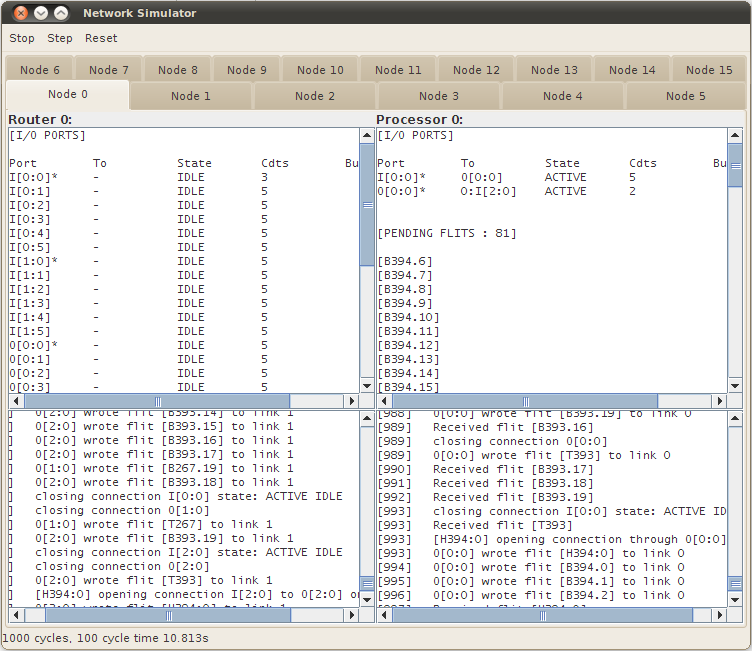
\includegraphics[scale=0.5]{debug.png}
\end{center}
\caption{Debug GUI}
\label{fig:debuggui}
\end{figure}

\subsubsection{Run Mode}

Run mode initialises the simulator to perform experiments. Run mode uses the
following extra parameters to specify the execution of the experiments.

\begin{paramlist}

\item[sim\_runs] Sets the number of complete simulation runs to be collated into
the final result.

\item[sample\_period] Sets the size of a sample period in cycles.

\item[num\_samples] Sets the number of samples to be taken, hence
\ttt{sample\_period} * \ttt{num\_samples} is the number of executed cycles used
for measurement. 

\item[latency\_thresh] Sets a threshold latency value in cycles. If the average
latency in the simulation exceeds this value then the simulation terminates. If
this value is set to 0 this it is disabled.

\item[warmup\_cycles] Sets the number of cycles necessary for the simulator to
reach a steady state. If this value is set to 0, then this is ignored and the
simulator warms up when the percentage change in latency and throughput is less
than the parameter \ttt{warmup\_thresh}.

\end{paramlist}

\subsection{Topology}

The \ttt{topology} parameter specifies the network topology and can take the
following values. The simulator supports two regular networks, the mesh and
torus, which also includes the hypercube, a special binary torus. It also
includes irregular constructions of mesh and tori by introducing a specific
level of link faults.

\begin{paramlist}

\item[mesh] A $k$-ary $n$-mesh, where $k$ and $n$ are specified by parameters
\ttt{k} and \ttt{n} respectively. 

\item[tori] A $k$-ary $n$-cube (torus), where $k$ and $n$ are specified by
parameters \ttt{k} and \ttt{n} respectively. A hypercube is specified as a 2-ary
$n$-cube.

\end{paramlist}


\subsection{Routing}

The \ttt{routing} parameter specifies the routing algorithm to be used in the
network and can take the following values. For each algorithm, some number of
virtual channels may be required to provide freedom from deadlock.

\begin{paramlist}

\item[dor] Dimension order routing, can only be used with mesh or torus
topologies. For meshes, only one virtual channel is necessary for deadlock
freedom. For tori, two virtual channels are necessary.

\item[updown] Up*/down* routing, compatible with any topology. The spanning tree
root node is randomly selected, or can be selected by setting \ttt{root\_node}
with a node identifier.

\item[minimal] Minimal path routing, used for debugging purposes, will deadlock.

\end{paramlist}


\subsection{Network}

The network parameters specify `physical' parameters of the network components.

\begin{paramlist}

\item[buffer\_size] Sets the size of the buffers in flits on input virtual channels.

\item[num\_vcs] Sets the number of virtual channels to use for each input
channel.

\item[link\_delay] Sets the number of cycles taken for flits and credits to be
transmitted along a link.

\item[rand\_seed] Sets the random number generator seed for the random elements
of network execution such as traffic generation.

\end{paramlist}


\subsection{Traffic}

The spatial distribution of traffic over the network is governed by a traffic
pattern, set using the \ttt{traffic\_pattern} parameter and can take the
following values:

\begin{paramlist}

\item[uniform] Each source sends a uniform amount of traffic to each other node.
Destination nodes are selected for each packet uniformly at random.

\item[bitcomp] Bit complement. $d_i = \neg s_i$

\item[bitrev] Bit reverse. $d_i = s_{b-i-1}$

\item[transpose] $d_i = s_{i+b/2 \mod b}$

\item[shuffle] $d_i = s_{i-1 \mod b}$

\item[tornado] $d_i = s_x + \lceil k/2 \rceil -1 \mod k$

\item[neighbour] $d_x = s_x + 1 \mod k$

\item[randperm] Random permutation. A fixed permutation of traffic is chosen
uniformly at random from the set of all permutations. The parameter
\ttt{perm\_seed} can be used to control randomness.

\end{paramlist}

The injection process determines the temporal distribution of traffic in the
network and is set with the \ttt{injection\_process} parameter and can take the
following values:

\begin{paramlist}

\item[bernoulli] Bernoulli injection process, the injection rate $r$ parameter
\ttt{injection\_rate} must be set such that $0< r \leq 1$.

\item[onoff] Modulated Markov Bernoulli process with two states `on' and `off'.
The probabilities of transitions between on and off $\alpha$ and $\beta$
respectively, can be set by \ttt{burst\_alpha} and \ttt{burst\_beta} such that $0
< \alpha, \beta \leq 1$.

\end{paramlist}

\noindent
Finally, the \ttt{flits\_per\_packet} parameter can be set to specify a
constant number of flits per packet.

\section{Extensibility}

The simulator has been designed and written in an object-orientated style as the
components of a network can intuitively be thought of as objects, for example
\ttt{Node} and \ttt{Link} objects constitute a \ttt{Network}. The simulator has
been designed to be an extensible platform that is non-specific to topologies or
routing algorithms, consequently the addition of new topologies or routing
algorithms is straight forward.

\subsection{Topologies}

A \ttt{Network} is a set of interconnected \ttt{Node}s. The static method
\ttt{Topology.createTopology()} is responsible for creating the set of
\ttt{Node}s. This can be done in two ways, the first is to create a
\ttt{Construction} graph which allows you to specify the topology by adding
edges between nodes to it. On completion, the \ttt{Construction} has a method
\ttt{create()} to create the set of \ttt{Node}s for the network.  The
code-snippet below shows how to randomly add edges between nodes to a
\ttt{Construction} and return the set of nodes.

\begin{egcode}
Construction graph = new Construction(numNodes);

for(int i=0; i<numNodes; i++) \{
    for(int j=0; j<numNodes; j++) \{
        if(rand.nextDouble < 0.5)
            graph.addEdge(i, j);
    \}
\}

Node[] nodes = graph.buildTopology();
\end{egcode}

The second, slightly more indirect way, is to explicitly construct the
\ttt{Node}s. This way is used for \ttt{Mesh} and \ttt{Torus} constructions as
greater control over the port constructions is necessary. To do this, each
\ttt{Node} must be constructed, then the \ttt{connectTo()} method can be used to
specify directional link connections. After all links have been connected the
\ttt{finishedConnecting()} must be called for each \ttt{Node}.  The code snippet
below shows how this type of construction could be used to build a ring.

\begin{egcode}
Node[] nodes = new Node[numNodes];

for(int i=0; i<nodes.length; i++)
    nodes[i] = new Node(i, 2, 2);

for(int i=0; i<numNodes; i++) \{
    nodes[i].connectTo(nodes[(i+1) % numNodes], 1, 2);
    nodes[i].connectTo(nodes[(i-1) % numNodes], 2, 1);
    nodes[i].finishConnecting();
\}
\end{egcode}

\noindent
For more examples, see the mesh and torus topologies included with the
simulator.

\subsection{Routing Algorithms}

New routing algorithms can be added to the simulator by implementing
the \ttt{RoutingFunction} interface. This specifies two methods to return an
output port and an output virtual channel based on the current node, the input
virtual channel and the destination node. Most of the algorithms implemented in
the simulator are based on tables, where lookups are performed to obtain output
ports and virtual channels. This requires a static configuration phase, and is
implemented with a static method in the routing function class called in the
\ttt{Network} object's constructor, passing in the \ttt{Network} object as an
argument.

\subsection{Experimentation}

Custom experiments should be built within the \ttt{RunMode} class.

\nocite{*}
\bibliographystyle{plain}
\bibliography{refs}

\end{document}
